\subsection{Casos de Uso del Recepcionista}
\label{subsec:casos_uso_recepcionista_general}

La figura \ref{fig:casos_uso_recepcionista} presenta los casos de uso que definen el comportamiento funcional del sistema desde la perspectiva del recepcionista. En este diagrama se identifican las interacciones relacionadas con la gestión, validación y canalización de las quejas recibidas.

\begin{figure}[H]
    \centering
    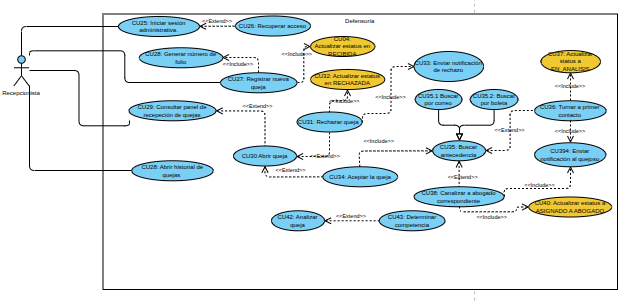
\includegraphics[width=0.9\textwidth]{imagenes/recepcion/Diagrama_CU/CasosUso_Recepcion.png}
    \caption{Diagrama de Casos de Uso del Microservicio Recepcionista}
    \label{fig:casos_uso_recepcionista}
\end{figure}

A continuación, se describen de manera detallada las especificaciones de los Casos de Uso representados, estableciendo los flujos estándar y las reglas de negocio que rigen la operación administrativa de la plataforma.

\vspace{0.5cm}